\section{Tangent-Linear/Adjoint Model Tests}
%===========================================
The tangent-linear/adjoint (TL/AD) test is a simpler one than the FWD/TL test. In this test both the CloudScatter and AerosolScatter tangent-linear and adjoint models are run with successive inputs given a value of 1.0. The subsequent TL output and transpose of the AD output should agree to within numerical precision. This should be true regardless of the LUT interpolation scheme used, and it was found to be so. The results shown here are simply an additional documentation of the difference between the adjoint model outputs that are due to the interpolation method.

\subsection{CloudScatter Module}
%-------------------------------
Using the snow cloud case for AMSU-A ch.8 again, the differences between the three interpolation methods  in the adjoint model is shown in figure \ref{fig:amsua_n18.ch8.SNOW.dOd_dReff.AD}. The Jacobian profile for the linear interpolation case, figure \ref{fig:amsua_n18.ch8.SNOW.dOd_dReff.AD}(a), is significantly different in shape and magnitude compared to either the cubic or averaged quadratic interpolation results. The differences between the cubic and averaged quadratic interpolation results are more subtle with the latter having a slightly larger peak value than the former.
\begin{figure}[htp]
  \centering
  \begin{tabular}{c c c}
    \multicolumn{3}{c}{\qquad\sffamily\textbf{NOAA-18 AMSU-A ch.8}}\\
    \multicolumn{3}{c}{\qquad\sffamily\textbf{Snow cloud test case}}\\
    \qquad\textsf{(a)} & \qquad\textsf{(b)}  & \qquad\textsf{(c)} \\
    \qquad\textsf{Linear} & \qquad\textsf{Cubic}  & \qquad\textsf{Averaged Quadratic} \\
    \includegraphics[bb=90 400 300 540,clip,scale=0.7]{graphics/Cloud/AD/amsua_n18.ch8.SNOW.NLIN.dOd_dReff.eps} &
    \includegraphics[bb=90 400 300 540,clip,scale=0.7]{graphics/Cloud/AD/amsua_n18.ch8.SNOW.NCUBIC.dOd_dReff.eps} &
    \includegraphics[bb=90 400 300 540,clip,scale=0.7]{graphics/Cloud/AD/amsua_n18.ch8.SNOW.AVGQUAD.dOd_dReff.eps} \\
  \end{tabular}
  \caption{Comparison of the tangent-linear (black) and adjoint (red) model optical depth variation with respect to effective radius profile for the NOAA-18 AMSU-A ch.8 snow cloud case using \textbf{(a)} linear, \textbf{(b)} cubic, and \textbf{(c)} averaged quadratic interpolation. See figure \ref{fig:Test.Profile4} for the snow cloud water content and effective radius profiles.}
  \label{fig:amsua_n18.ch8.SNOW.dOd_dReff.AD}
\end{figure}

A similar comparison for the rain cloud case for AMSU-A channel 15 is shown in figure \ref{fig:amsua_n18.ch15.RAIN.dw_dReff.AD}. In this example, the case of figure \ref{fig:amsua_n18.ch15.RAIN.dw_dReff.AD}(a) clearly shows the shortcomings of using linear interpolation with the current cloud optical property LUT data. Comparison of the cubic and averaged quadratic interpolation results of figure \ref{fig:amsua_n18.ch15.RAIN.dw_dReff.AD}(b) and (c) respectively again shows subtle, but noticeable, differences in both the Jacobian shape and peak magnitudes.
\begin{figure}[htp]
  \centering
  \begin{tabular}{c c c}
    \multicolumn{3}{c}{\qquad\sffamily\textbf{NOAA-18 AMSU-A ch.15}}\\
    \multicolumn{3}{c}{\qquad\sffamily\textbf{Rain cloud test case}}\\
    \qquad\textsf{(a)} & \qquad\textsf{(b)}  & \qquad\textsf{(c)} \\
    \qquad\textsf{Linear} & \qquad\textsf{Cubic}  & \qquad\textsf{Averaged Quadratic} \\
    \includegraphics[bb=90 400 300 540,clip,scale=0.7]{graphics/Cloud/AD/amsua_n18.ch15.RAIN.NLIN.dw_dReff.eps} &
    \includegraphics[bb=90 400 300 540,clip,scale=0.7]{graphics/Cloud/AD/amsua_n18.ch15.RAIN.NCUBIC.dw_dReff.eps}  &
    \includegraphics[bb=90 400 300 540,clip,scale=0.7]{graphics/Cloud/AD/amsua_n18.ch15.RAIN.AVGQUAD.dw_dReff.eps} \\
  \end{tabular}
  \caption{Comparison of the tangent-linear (black) and adjoint (red) model single scatter albedo variation with respect to effective radius profile for the NOAA-18 AMSU-A ch.15 rain cloud case using \textbf{(a)} linear, \textbf{(b)} cubic, and \textbf{(c)} averaged quadratic interpolation. See figure \ref{fig:Test.Profile3} for the rain cloud water content and effective radius profiles.}
  \label{fig:amsua_n18.ch15.RAIN.dw_dReff.AD}
\end{figure}

 
\subsection{AerosolScatter Module}
%---------------------------------
The NOAA-18 HIRS/4 sea salt (SSAM) test case discussed in the FWD/TL section, as well as a dust aerosol case, are shown here. The results for single scatter albedo and asymmetry parameter Jacobian profiles for the three interpolation schemes are shown in figures \ref{fig:hirs4_n18.ch8.SSAM.dw_dReff.AD} and \ref{fig:hirs4_n18.ch8.DUST.dg_dReff.AD} for the sea salt (SSAM) and dust aerosol cases respectively. The differences between the results due to the interpolation is not as marked for the aerosol cases as for the cloud cases - probably due to a combination of a smaller radiometric effect in general for aerosols, and a higher LUT data density that tends to minimise interpolation errors.

\begin{figure}[htp]
  \centering
  \begin{tabular}{c c c}
    \multicolumn{3}{c}{\qquad\sffamily\textbf{NOAA-18 HIRS/4}}\\
    \multicolumn{3}{c}{\qquad\sffamily\textbf{Sea salt (SSAM) test case}}\\
    \qquad\textsf{(a)} & \qquad\textsf{(b)}  & \qquad\textsf{(c)} \\
    \qquad\textsf{Linear} & \qquad\textsf{Cubic}  & \qquad\textsf{Averaged Quadratic} \\
    \includegraphics[bb=90 400 300 540,clip,scale=0.7]{graphics/Aerosol/AD/hirs4_n18.ch8.SSAM.NLIN.dw_dReff.eps} &
    \includegraphics[bb=90 400 300 540,clip,scale=0.7]{graphics/Aerosol/AD/hirs4_n18.ch8.SSAM.NCUBIC.dw_dReff.eps} &
    \includegraphics[bb=90 400 300 540,clip,scale=0.7]{graphics/Aerosol/AD/hirs4_n18.ch8.SSAM.AVGQUAD.dw_dReff.eps}
  \end{tabular}
  \caption{Comparison of the tangent-linear (black) and adjoint (red) model single scatter albedo variation with respect to effective radius profile for the NOAA-18 HIRS/4 ch.8 sea salt (SSAM) aerosol case using \textbf{(a)} linear, \textbf{(b)} cubic, and \textbf{(c)} averaged quadratic interpolation. See figure \ref{fig:Test.Profile2} for the sea salt (SSAM) aerosol concentration and effective radius profiles.}
  \label{fig:hirs4_n18.ch8.SSAM.dw_dReff.AD}
\end{figure}

\begin{figure}[htp]
  \centering
  \begin{tabular}{c c c}
    \multicolumn{3}{c}{\qquad\sffamily\textbf{NOAA-18 HIRS/4}}\\
    \multicolumn{3}{c}{\qquad\sffamily\textbf{Dust test case}}\\
    \qquad\textsf{(a)} & \qquad\textsf{(b)}  & \qquad\textsf{(c)} \\
    \qquad\textsf{Linear} & \qquad\textsf{Cubic}  & \qquad\textsf{Averaged Quadratic} \\
    \includegraphics[bb=90 400 300 540,clip,scale=0.7]{graphics/Aerosol/AD/hirs4_n18.ch8.DUST.NLIN.dg_dReff.eps} &
    \includegraphics[bb=90 400 300 540,clip,scale=0.7]{graphics/Aerosol/AD/hirs4_n18.ch8.DUST.NCUBIC.dg_dReff.eps} &
    \includegraphics[bb=90 400 300 540,clip,scale=0.7]{graphics/Aerosol/AD/hirs4_n18.ch8.DUST.NCUBIC.dg_dReff.eps} \\
  \end{tabular}
  \caption{Comparison of the tangent-linear (black) and adjoint (red) model asymmetry parameter variation with respect to effective radius profile for the NOAA-18 HIRS/4 ch.8 dust aerosol case using \textbf{(a)} linear, \textbf{(b)} cubic, and \textbf{(c)} averaged quadratic interpolation. See figure \ref{fig:Test.Profile1} for the dust aerosol concentration and effective radius profiles.}
  \label{fig:hirs4_n18.ch8.DUST.dg_dReff.AD}
\end{figure}

